\section{Abläufe}

Während in Kapitel 2 die Interaktion der Hauptkomponenten \emph{Server} und der \emph{RobotUnit} abgehandelt wurden, werden im Folgenden die Abläufe der Use Cases genauer spezifiziert und auch interne Komponentenabläufe beschrieben, im Speziellen die Abläufe innerhalb der \emph{RobotUnit}.
	
	\subsection*{Interaktion bei Ausführung von Use Case 1 – \emph{Choose Path around Obstacle} und Use Case 2 – \emph{Drive around Obstacle}}
	Sowohl der Use Case \emph{Choose Path around Obstacle} als auch der Use Case \emph{Drive around Obstacle} sind beide Teil des Geschäftsprozesses \emph{Drive to Destination}. Abbildung \ref{UmfahrenvonstatichenObjekten} zeigt ein Sequenzdiagramm des Use Case \emph{Drive around Obstacle}. Wie schon der Name beschreibt, befindet sich die \emph{RobotUnit} dabei in einem Fahrvorgang, der vorher konkret mit der Zielposition und der Geschwindigkeit vom \emph{Server} eingestellt wurde. 
	
	So reagiert intern seine Software mit dem \emph{IDistanceSensor}, wenn ein Hindernis um ihn herum auftaucht und dieses mit Hilfe der durch die Sensoren gesammelten Informationen umfahren werden muss. Dabei muss der \emph{Robot} ausdrücklich zwischen einem \emph{Robot} und einem unbeweglichen Hindernis unterscheiden, um so vorherzubestimmen, wie eine optimale Ausweichbewegung aussieht. Auch wenn der \emph{IDistanceSensor} die vollständige Umgebung um den \emph{Robot} wahrnehmen kann, bezieht sich dies jedoch primär auf vor dem \emph{Robot} liegende Hindernisse. Dieser Prozess ist Bestandteil des Use Case \emph{Choose Path around Obstacle} und geht dann in den Use Case \emph{Drive Around Obstacle} über. 
	
	Der \emph{Robot} koordiniert sich dort mit seiner \emph{IDrive}-Komponente und seinen Sensoren, um langsam an einem unbeweglichen Objekt vorbeizufahren. Dabei fährt er immer eine kleine Distanz parallel zur Kante des \emph{Obstacles} und prüft, ob der Weg zum Ziel wieder frei ist. Ist dies der Fall, nimmt er den Fahrtprozess wieder auf. Erkennen sich zwei \emph{Robots} hingegen gegenseitig als Hindernis, weichen beide mit Hilfe ihrer \emph{IDrive}-Komponente jeweils nach rechts aus und nehmen anschließend den normalen Fahrbetrieb wieder auf. \\
	
	\subsection*{Interaktion bei Ausführung von Use Case 3 – \emph{Read Sensors}}
In Abbildung \ref{ReadSensors} wird der reine Anfrageprozess zwischen \emph{Server} und der \emph{RobotUnit} aus Kapitel 2 erweitert. Nach der Anfrage wird der \emph{Robot} alle nötigen Informationen nacheinander abfragen: Sowohl die \emph{Position} als auch die Orientierungsrichtung werden von der \emph{INorthStar}-Komponente zurückgeliefert. Für den Batteriestatus muss die \emph{IBattery}-Komponente angefragt werden. Erst wenn alle Informationen als Gesamtpaket bereitstehen, können sie an den Server zurückgemeldet werden.
\\
	\begin{figure}[H]
		\centering
		\includegraphics[width=0.95\textwidth]{img/1-Entwurf-8-DriveArroundObstacle}
		\caption{Sequenzdiagramm von \emph{Drive arround Obstacle}}
		\label{UmfahrenvonstatichenObjekten}
	\end{figure}
	\vspace{1cm}
	
	\begin{figure}[H]
		\centering
		\includegraphics[width=1\textwidth]{img/0-Entwurf-8-ReadSens}
		\caption{Sequenzdiagramm von \emph{Read Sensors}}
		\label{ReadSensors}
	\end{figure}
	
	
	
	\subsection*{Interaktion bei Ausführung von Use Case 4 – \emph{Charging}}
	Beim Use Case \emph{Charging} (Sequenzdiagramm in Abbildung \ref{Charging}) findet keine Kommunikation mit der Komponente \emph{Server} statt, dafür allerdings zwischen der \emph{RobotUnit} und der \emph{Charging\-Station}. Hat der \emph{Robot} einen bestimmten kritischen Ladestand erreicht (den er regelmäßig überprüft), läuft er die \emph{Charging\-Station}-Komponente an. Der Ladevorgang triggert automatisch, sobald der \emph{Robot} die \emph{Position} der Ladestation erreicht hat, und interagiert solange mit ihr bis seine Batterie wieder aufgeladen ist. Innerhalb des \emph{Robots} werden zum Anfahren der \emph{ChargingStation} die Komponenten \emph{IBattery} mit der \emph{Position} der robotereigenen Ladestation und \emph{IDrive} benötigt. Konkret: Wenn \emph{IDrive} \texttt{arrived()} zurückgibt, kann der Ladevorgang begonnen werden.
	\vspace{1cm}
	
	\begin{figure}[H]
		\centering
		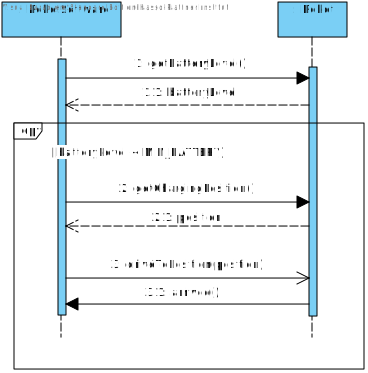
\includegraphics[width=0.65\textwidth]{img/0-Entwurf-8-Charging}
		\caption{Sequenzdiagramm von \textit{Charging}}
		\label{Charging}
	\end{figure}
